\documentclass[fleqn, twocolumn]{article}
\usepackage{amsmath, tikz}

\title{Resolução de Exercícios Cálculo 2}
\author{Lázaro Jośe Rodrigues Júnior}

\begin{document}

    \maketitle
    
    \section{Lista I}
    \subsection{Substituição Trigonométrica}   
    \[1) \int \frac{dx}{x^2 \sqrt{4-x^2}}  \]
    Colocando o 4 em evidência;
        \[ \int \frac{dx}{x^2 \sqrt{4(1-{(\frac{x}{2}})^2)}}\]
    Seja $\frac{x}{2} = \sin{t}$ , $x = 2 \sin{t}$ , $ dx = 2\cos{t}\ dt$ ;
        \[ \int \frac{2\cos{t}\ dt}{(2\sin{t})^2 \sqrt{4(1-{\sin^2{t}})}}\]
    Como $1-\sin^2{t} = \cos^2{t}$;
        \[ \int \frac{2\cos{t}\ dt}{4\sin^2{t}\ 2\cos{t}} \]
    Simplificando;
        \[\frac{1}{4}\int \csc^2{t}\ dt \]
    Integrando;
        \[-\frac{1}{4}\cot{t} + c\]
    Como $\frac{x}{2} = \sin{t}$:
 
    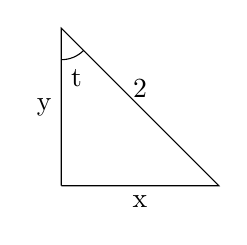
\begin{tikzpicture}[scale=2]
        \draw (0,0) -- (0,1)node[midway, left]{y}
             -- (1,0)node[midway, above]{2} -- (0,0)node[midway, below]{x};
        \draw (0,0.8)node[below right]{t} 
            arc [start angle=270, end angle=315, radius=2mm];
    \end{tikzpicture}

    Como precisamos encontrar a cotangente $(\frac{cateto\ adjantece}{cateto\ oposto})$, precisamos encontrar o y, e pelo teorema
de pitágoras: $2^2 = x^2 + y^2$, isolando o y: $y = \sqrt{4-x^2}$.
   
    Logo a resposta final é: \[-\frac{\sqrt{4-x^2}}{4x} +c\]

    \[2) \int \frac{dx}{x \sqrt{x^2+4}}  \]
    Colocando o 4 em evidência;
        \[ \int \frac{dx}{x \sqrt{4((\frac{x}{2})^2 + 1)}}\]
    Seja $\frac{x}{2} = \tan{t}$ , $x = 2 \tan{t}$ , $ dx = 2\sec^2{t}\ dt$;
        \[ \int \frac{2\sec^2{t}\ dt}{2 \tan{t} \sqrt{4(\tan^2{t} + 1)}}\]
    Como $\tan^2{t}+1 = \sec^2{t}$;
        \[ \int \frac{2\sec^2{t}\ dt}{2\tan{t}\ 2\sec{t}} \]
    Simplificando;
        $\frac{1}{2}\int \frac{\sec{t}}{\tan{t}}$
    =
        $\frac{1}{2}\int \frac{\frac{1}{\cos{t}}}{\frac{\sin{t}}{\cos{t}}}$
    =
        $\frac{1}{2}\int \frac{1}{\sin{t}}$
    =
        \[\frac{1}{2}\int \csc{t}\]
    Integrando;
        \[-\ln(\csc{t}+\cot{t})+c\]
    \newpage

    Como $\frac{x}{2} = \tan{t}$:

    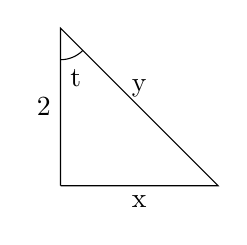
\begin{tikzpicture}[scale=2]
        \draw (0,0) -- (0,1)node[midway, left]{2}
             -- (1,0)node[midway, above]{y} -- (0,0)node[midway, below]{x};
        \draw (0,0.8)node[below right]{t} 
            arc [start angle=270, end angle=315, radius=2mm];
    \end{tikzpicture}

    Como precisamos encontrar a cotangente $(\frac{cateto\ adjantece}{cateto\ oposto})$ e a cosecante $(\frac{hipotenusa}{cateto\ oposto})$, precisamos encontrar o y, e pelo teorema
de Pitágoras: $y^2 = x^2 + 2^2$, isolando o y: $y = \sqrt{x^2 +4}$.
   
    Logo a resposta final é: \[-\ln(\frac{\sqrt{x^2 +4}}{x} + \frac{2}{x})+c \]

    \[3) \int \frac{dx}{x \sqrt{25-x^2}}  \]
    Colocando o 25 em evidência;
        \[ \int \frac{dx}{x \sqrt{25(1-{(\frac{x}{5}})^2)}}\]
    Seja $\frac{x}{5} = \sin{t}$ , $x = 5 \sin{t}$ , $ dx = 5\cos{t}\ dt$ ;
        \[ \int \frac{5\cos{t}\ dt}{(5\sin{t}) \sqrt{25(1-{\sin^2{t}})}}\]
    Como $1-\sin^2{t} = \cos^2{t}$;
        \[ \int \frac{5\cos{t}\ dt}{5 \sin{t}\ 5\cos{t}} \]
    Simplificando;
        \[\frac{1}{5}\int \csc{t}\ dt \]
    Integrando;
        \[-\frac{1}{5} \ln(\csc{t} + \cot{t}) + c\]
    Como $\frac{x}{5} = \sin{t}$:
 
    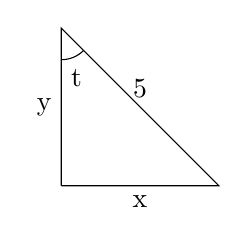
\begin{tikzpicture}[scale=2]
        \draw (0,0) -- (0,1)node[midway, left]{y}
             -- (1,0)node[midway, above]{5} -- (0,0)node[midway, below]{x};
        \draw (0,0.8)node[below right]{t} 
            arc [start angle=270, end angle=315, radius=2mm];
    \end{tikzpicture}

    Como precisamos encontrar a cosecante $(\frac{hipotenusa}{cateto\ oposto})$ e a cotangente $(\frac{cateto\ adjantece}{cateto\ oposto})$, precisamos encontrar o y, e pelo teorema
de Pitágoras: $5^2 = x^2 + y^2$, isolando o y: $y = \sqrt{25-x^2}$.
   
    Logo a resposta final é: \[-\frac{1}{5} \ln( \frac{5}{x} + \frac{\sqrt{25-x^2}}{x} ) +c\]

\end{document}
